\documentclass[60pt]{article}

\title{Informe}
%%------------ Paquetes utilizados
\usepackage[utf8]{inputenc} %Indica qué codificación se está usando ISO-8859-1(latin1)  o utf8  
\usepackage[spanish]{babel}%Indica que escribiermos en español
%\usepackage{amsmath} % Comandos extras para matemáticas (cajas para ecuaciones,
% etc)
%\usepackage{amssymb} % Simbolos matematicos (por lo tanto)
\usepackage{graphicx} % Incluir imágenes en LaTeX
\usepackage{color} % Para colorear texto
%\usepackage{subfigure} % subfiguras
\usepackage{float} %Podemos usar el especificador [H] en las figuras para que se
% queden donde queramos
\usepackage{algorithm,algpseudocode}%para crear algoritmos
\usepackage{capt-of} % Permite usar etiquetas fuera de elementos flotantes
% (etiquetas de figuras)
\usepackage{sidecap} % Para poner el texto de las imágenes al lado
    \sidecaptionvpos{figure}{c} % Para que el texto se alinie al centro vertical
\usepackage{caption} % Para poder quitar numeracion de figuras
\usepackage{subcaption}
%\usepackage{commath} % funcionalidades extras para diferenciales, integrales,
% etc (\od, \dif, etc)
%\usepackage{cancel} % para cancelar expresiones (\cancelto{0}{x})
\usepackage{anysize}                    % Para personalizar el ancho de  los márgenes
\marginsize{2cm}{2cm}{2cm}{2cm} % Izquierda, derecha, arriba, abajo
\usepackage{appendix}
\usepackage{fancyhdr} %Personalizar encabezado y pie de página
\usepackage{listingsutf8} % Para usar código fuente
\usepackage{parcolumns}
\usepackage{blindtext}
\usepackage{float}
\usepackage[
backend=biber,
style=alphabetic,
sorting=ynt
]{biblatex}
\addbibresource{bibliografias.bib}


%%------------ Redefinición de Comandos
\renewcommand{\appendixname}{Anéxos}
\renewcommand{\appendixtocname}{Anéxos}
\renewcommand{\appendixpagename}{Anéxos} 
\newcommand*\sepline{%
    \begin{center}
        \rule[1ex]{.5\textwidth}{.5pt}
    \end{center}
    }

\usepackage{glossaries}

\makeglossaries
    
    

\newglossaryentry{patrón}
{
    name=patrón,
    description={Conjunto de cartas que se deben completar.}
}
\newglossaryentry{baraja}
{
    name=baraja,
    description={Conjunto de cartas que se utilizan en el juego.}
}
\newglossaryentry{descarte}
{
    name=descarte,
    description={Conjunto de cartas que se han retirado de la baraja.}
}
\newglossaryentry{mano}{
    name=mano,
    description={Conjunto de cartas que se tienen en la mano.}
}

%Comandos  definidos para la plantilla
\newcommand{\university}{Universidad Católica de la Santísima Concepción}
\newcommand{\universityshort}{UCSC}
\newcommand{\faculty}{Facultad de Ingeniería}
\newcommand{\depto}{Ingeniería Civil Informática}
\newcommand{\class}{Taller de programación II}
\newcommand{\classcode}{N1069C/1}
\newcommand{\Title}{Carioca}
\newcommand{\Author}{
David Gómez Pinto

Lucas Ayala Casanova}
\newcommand{\teacher}{Diego Maldonado Montiel}
\newcommand{\Date}{17 de octubre de 2022}%Aquí ingrese la fecha de entrega (\today inserta la fecha actual)
\renewcommand{\lstlistingname}{Fragmento}% Listing -> Fragmento
\floatname{algorithm}{Algoritmo}%algorithm->Algotimo
%%------------ Configuraciones específicas de paquetes

%%-------- Color y Referencias
% Para que las referencias sean hipervínculos a las figuras o ecuaciones y
% aparezcan en color
\usepackage[colorlinks=false,plainpages=true,citecolor=blue,linkcolor=blue]{hyperref}
%\usepackage{hyperref} 


%%-------- Personalizar encabezado y pie de página
\pagestyle{fancy}
%%-- Portada
\fancypagestyle{mytitlepagestyle}{%
	\renewcommand{\headrulewidth}{0pt}
	\fancyhead[L]{
		
\includegraphics[width=6cm]{images/template/logo_facultad.png}
	}
}
%%-- Páginas
\fancypagestyle{mypagestyle}{%
	\fancyhf{}
	\fancyhead[L]{\footnotesize \universityshort} %encabezado izquierda
	\fancyhead[R]{\footnotesize \faculty}   % dereecha
	\fancyfoot[L]{\footnotesize \depto}  % Pie izquierda
	\fancyfoot[R]{\footnotesize \class}  % Pie derecha
	\fancyfoot[C]{\thepage}  % centro%\fancyfoot[L]{\footnotesize Estándares de desarrollo}  %izquierda
	\renewcommand{\footrulewidth}{0.4pt}
}


%%-------- Personalizar código fuente

\definecolor{dkgreen}{rgb}{0,0.6,0} % Definimos colores para usar en el código
\definecolor{gray}{rgb}{0.5,0.5,0.5} 
% configuración para el lenguaje que queramos utilizar

\definecolor{codegreen}{rgb}{0,0.6,0}
\definecolor{codegray}{rgb}{0.5,0.5,0.5}
\definecolor{codepurple}{rgb}{0.58,0,0.82}
\definecolor{backcolour}{rgb}{0.95,0.95,0.92}
\lstdefinestyle{mystyle}{
	backgroundcolor=\color{backcolour},
	frame=single, 
	commentstyle=\color{codegreen},
	keywordstyle=\color{magenta},
	numberstyle=\tiny\color{codegray},
	stringstyle=\color{codepurple},
	basicstyle=\ttfamily\footnotesize,
	breakatwhitespace=false,         
	breaklines=true,                 
	captionpos=b,                    
	keepspaces=true,                 
	numbers=left,                    
	numbersep=5pt,                  
	showspaces=false,                
	showstringspaces=false,
	showtabs=false,                  
	tabsize=2
}

\lstset{style=mystyle}


\title{Plantilla para informes de tarea}
%---------------------------------------------------------------------------------------

\begin{document}
\thispagestyle{mytitlepagestyle}
%%%%%%%%%%%%%%%%%%%%%%%%%%%%%%%%%% PORTADA %%%%%%%%%%%%%%%%%%%%%%%%%%%%%%%%%%%%%%%%%%%%
\thispagestyle{mytitlepagestyle}													%%%
\noindent	                                                                        %%%
\begin{center}                                                                      %%%
    %%%
    \vspace*{0.8cm}																		%%%
    %%%
    \begin{minipage}{0.9\textwidth} 													%%%
        \begin{center}																	%%%
            \textsc{\huge \uppercase{\depto}}\\[0.5cm]  						%%%
            \textsc{\Large \class}\\[1.5cm] 								%%%
        \end{center}																	%%%
    \end{minipage}\\[0.5cm]																%%%
    %%%
    \vspace*{\fill}																		%%%
    %%%                       
    %%{ \Large  \preTitle}\\[0.2cm]															%%%
    { \Huge \bfseries \Title}\\[0.4cm]										%%%
    %%%
    \vspace*{\fill}																		%%%
    %%%
    \begin{minipage}{0.46\textwidth}                                                    %%%
        \begin{flushleft} \large                                                            %%%
            \emph{Autor:}\\   																	%%%
            \Author\\																	%%%
            %%%
        \end{flushleft}                                                                     %%%
    \end{minipage}
    %%%
    \begin{minipage}{0.52\textwidth}
        \vspace{-0.6cm}                                         %%%
        \begin{flushright} \large                                                           %%%
            \emph{Profesor:} \\                                                                 %%%
            \teacher\\                                                   %%%
        \end{flushright}                                                                    %%%
    \end{minipage}
    \vspace*{1cm}
    %\begin{flushleft}
    %\end{flushleft}
    %%%
    %%        \flushleft{\textbf{\Large Ing. Mecatrónica} }\\                                                                     %%%
    \vspace*{\fill}
    \begin{center}
        {\large \Date}                                                                 %%%
    \end{center}
\end{center}

\newpage
%%%%%%%%%%%%%%%%%%%% TERMINA PORTADA %%%%%%%%%%%%%%%%%%%%%%%%%%%%%%%%
\pagestyle{mypagestyle}
%%------------  Tabla de contenidos ó índice (Se genera solo a partir de las secciones que creen)
\tableofcontents

\newpage
%%------------  Comience a editar aquí su documento



\section{Introducción.}\label{cap:intro}

En el presente documento se procedera a realizar un análisis a profundidad de la propuesta de software para el determinado juego de mesa: Cariocas. En el cual se detallaran los procedimientos que se ejecutan a nivel de sistema para luego facilitar el uso del usuario final (en adelante llamado jugador).



\subsection{Próposito del Sistema.}\label{cap:proposito}
Proveer de un entorno integral con tal de que el jugador logre competir contra otros de manera justa, correcta e imparcial ante el sistema con el cual el jugador pueda disfrutar de la entretención que entrega el presente juego de cartas.

\subsection{Alcance del Sistema.}\label{cap:alcance}
El sistema se va a encargar de implementar la logica y reglas del juego de tal forma que el jugador pueda interactuar con este a traves de una interfaz grafica

\subsection{Objetivos y criterios de éxito del proyecto.}\label{cap:objetivos}
Garantizar la correcta resolución del juego, libre de errores y contratiempos que afecten la dinámica de este.

Proporcionar un sistema el cual sea fácil e intuitivo de seguir y usar.

Entregar un sistema en el que ningún jugador se vea beneficiado más allá de las reglas del juego.
\subsection{Definiciones, siglas y abreviaturas.}\label{cap:definiciones}
Pinta - Símbolos que agrupan un determinado tipo de carta, entre ellas existen los siguientes grupos: Picas, Corazones, Rombos y Tréboles.

Trio - Agrupación de tres cartas de un mismo valor númerico.

Escala - Secuencia de cuatro cartas de una misma pinta y con valor númerico ascendente.

Escala Real - Secuencia de doce cartas de una misma pinta y un valor númerico ascendente, corresponden a todas las cartas de la misma pinta exceptuando las cartas Joker.

Jack (J) - Corresponde a la primera carta proveniente después de la carta número diez.

Queen (Q) - Corresponde a la segunda carta proveniente después de la carta número diez.

Kaiser (K) - Corresponde a la tercera carta proveniente después de la carta número diez.

Joker - Es una carta comodín la cual puede adquirir cualquier valor númerico según el jugador estipule. Además, si el juego es en base a puntaje, esta carta tiene más puntaje. Para más información leer reglas del juego estipuladas en el presente documento.
\subsection*{Referencias}
\begin{itemize}
    \item Las referencias utilizadas en este informe provienen de \textit{Ingeniería de software orientado a objetos. Bruegge,Bernd y Dutoit,Allen H.} \cite{oop}
\end{itemize}
\section{Sistema Actual.}\label{cap:sistemaActual}
En la actualidad no existe un sistema que permita jugar Cariocas de manera digital. Por lo tanto, el sistema que se propone es el primero en su tipo.
\section{Sistema propuesto.}\label{cap:sistema}
\subsection{Panorama.}\label{cap:panorama}
El sistema permite al usuario realizar las operaciones básicas del juego de una forma eficaz y libre de errores, las cuales consisten en acciones relacionadas al retirar carta de la \gls{baraja}, bajar mano, entre otras relacionadas. El sistema se deberá se desarrollar en Python 3 por lo que contará con una interfaz en base a linea de comandos. Contará con una base de datos interna que logrará que los datos estén de manera persistente en el sistema, independientemente si la energia del hardware deja de ser suministrada o no.
\subsection{Requerimientos Funcionales.}\label{cap:requerimientos-funcionales}
Las Cariocas son un juego de cartas en el cual consiste en reunir un determinado \gls{patrón} de cartas basado en su valor númerico o en sus pintas. Para el inicio del juego es menester disponer de una \gls{baraja} de cartas y una cantidad de 1 a 6 jugadores que deben ser ingresados en el sistema almacenados en una estructura de datos interna la cual se utilizará para una correcta resolución de las rondas del juego. 

A cada jugador se le debe brindar 12 cartas aleatoriamente las que deberá analizar durante su turno. Los turnos de los jugadores inician cuando el jugador en cuestión retira una carta de la \gls{baraja} y son finalizados cuando este descarta una carta elegida por el mismo, de su mano actual.

Al lograr reunir el patrón\Gls{patrón} de cartas exigidos por la ronda, el jugador requiere lograr bajar ese determinado \gls{patrón}, puede ser un Trio, una Escala o una Escala Real, el termino bajar consiste en poner los patrones solicitados con el dorso de las cartas boca abajo para que las pintas puedan ser vistas por otros jugadores.

Cuando un jugador realiza la acción anterior, si los otros jugadores han realizado el mismo procedimiento, ellos pueden botar una carta que correspondiente al \gls{patrón} exigido por la ronda.

Cabe destacar que cuando se baja un jugador, este no podrá botar cartas en el mismo turno, por lo que si el jugador no logra bajar en su turno, deberá esperar a que los otros jugadores hayan realizado su acción para poder bajar.

Las rondas estan definidas por el patrón que se necesita a medida que avanza el juego. El \gls{patrón} es de carácter progresivo y la cantidad de rondas oficiales son 9.

El jugador, si lo desea, puede abandonar el juego al terminar la ronda.
\subsection{Requerimientos No Funcionales.}\label{cap:requerimientos-no-funcionales}
El juego de cariocas debe mantener una persistencia temporal de datos, la cual está administrada por la memoria RAM y sufre las mismas limitaciones de esta (por ejemplo,almacenamiento limite definido por el hardware, al apagar el equipo se pierde la información).  El tiempo de respuesta esta definido por el lenguaje en el cual se desarrollará el sistema.

\subsection{Seudorrequerimientos.}\label{cap:seudorrequerimientos}
El software debe estar desarrollado únicamente en Python 3 por solicitud del cliente.
\subsection{Modelos del sistema.}\label{cap:modelos-sistema}

\subsection{Escenarios.}\label{cap:escenarios}

%Escenario
\begin{center}
    \begin{tabular}{ l | c  }
        Nombre del escenario: & Realización Típica de Turnos \\
        Instancia actores participantes: & Jugador: Usuario \\\hline
        Flujo de eventos: &  1.-Cada jugador recibe 12 cartas\\
        & 2.-El jugador retira una carta de la \gls{baraja}\\   
        & 3.-El jugador analiza su mano y descarta una carta\\  
        & 4.-Se procede al siguiente turno iterando nuevamente la secuencia\\
        & 5.-Si alguno completa el \gls{patrón} solicitado por la ronda,\\
        & entonces baja su mano\\
        & 6.-Si el jugador baja su mano, entonces no podrá botar \\
        & cartas en el mismo turno\\
        & 7.-Cuando le toque nuevamente su turno, el jugador podrá botar cartas\\
        & 8.-La ronda termina cuando un jugador tiene una sola carta\\
        & y este finaliza su turno al descartar su última carta\\
        & 9.-El juego termina cuando se han completado las 9 rondas oficiales\\
        \hline
    \end{tabular}
\end{center}
\subsubsection{Modelos de casos de uso.}\label{cap:modelos-casos-uso}
\clearpage
\begin{figure}[h]
    \centering
    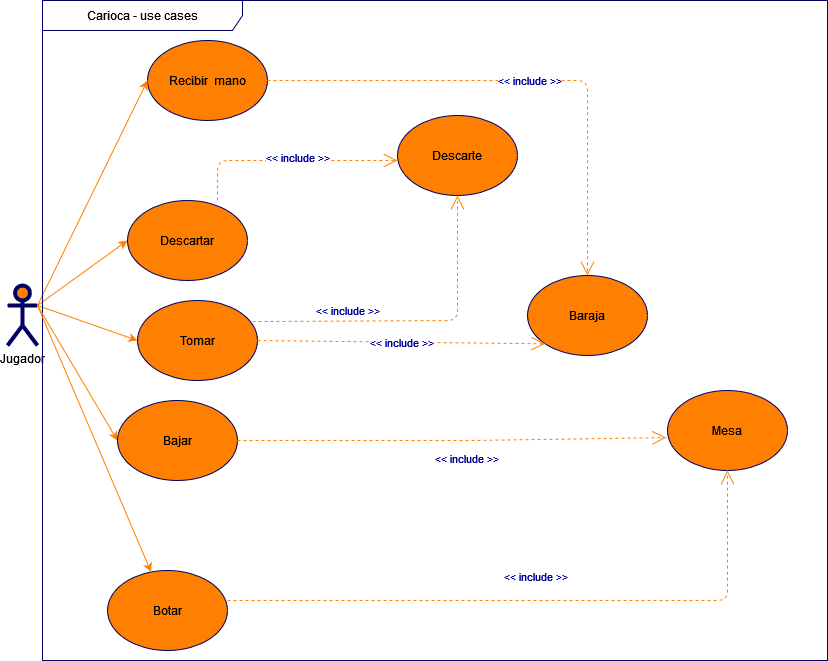
\includegraphics[width=15cm]{use-cases.png}
    \caption{Diagrama de casos de uso generalizado.}
\end{figure}
%CASO DE USO 1
\begin{center}
    \begin{tabular}{ l | c  }
        Nombre del caso de Uso: & Recibir mano \\
        Actor participante: & Iniciado por: Jugador \\\hline
        Condicion Inicial: & 1. Debe ser la primera ronda    \\
        Flujo de eventos: & 2. El jugador recibe 12 cartas aleatoriamente \\\hline
        Condicion de Salida: & 3. Se muestra en pantalla el turno del jugador \\
        & 4. Se muestra en pantalla el Total de Cartas: N \\
        & 5. Se muestra en pantalla Cartas en la mesa \\
        & 6. Se muestra en pantalla Cartas en descartes\gls{Descarte} \\
        & 7. Se muestra en pantalla Cartas en la mano \\
        & 8. Se muestra en pantalla un menu de opciones \\ 
    \end{tabular} \\
\end{center}
%FIN CASO DE USO 1
%CASO DE USO 2
\begin{center}
    \begin{tabular}{ l | c  }
        Nombre del caso de Uso: & Retirar carta de la \gls{baraja} \\
        Actor participante: & Iniciado por: Jugador \\\hline
        Condicion Inicial: & 1. Debe ser el turno del jugador    \\
        Flujo de eventos: & 2. El jugador retira una carta de la \gls{baraja} \\\hline
        Condicion de Salida: & 3. Se muestra en pantalla la carta retirada \\
        & 4. Se muestra en pantalla el turno del jugador \\
        & 5. Se muestra en pantalla el Total de Cartas: N \\
        & 6. Se muestra en pantalla Cartas en la mesa \\
        & 7. Se muestra en pantalla Cartas en descartes \\
        & 8. Se muestra en pantalla Cartas en la mano \\
        & 9. Se muestra en pantalla un menu de opciones \\ 
    \end{tabular} \\
\end{center}
%FIN CASO DE USO 2
%CASO DE USO  3
\begin{center}
    \begin{tabular}{ l | c  }
        Nombre del caso de Uso: & Descartar carta de la mano \\
        Actor participante: & Iniciado por: Jugador \\\hline
        Condicion Inicial: & 1. Debe ser el turno del jugador    \\
        Flujo de eventos: & 2. El jugador descarta una carta de su mano \\\hline
        Condicion de Salida: & 3. Se muestra en pantalla la carta descartada \\
        & 4. Se muestra en pantalla el turno del jugador \\
        & 5. Se muestra en pantalla el Total de Cartas: N \\
        & 6. Se muestra en pantalla Cartas en la mesa \\
        & 7. Se muestra en pantalla Cartas en descartes \\
        & 8. Se muestra en pantalla Cartas en la mano \\
        & 9. Se muestra en pantalla un menu de opciones \\ 
    \end{tabular} \\
\end{center}
%FIN CASO DE USO 3
%CASO DE USO 4
\begin{center}
    \begin{tabular}{ l | c  }
        Nombre del caso de Uso: & Bajar \Gls{patrón} \\
        Actor participante: & Iniciado por: Jugador \\\hline
        Condicion Inicial: & 1. Debe ser el turno del jugador    \\
        Flujo de eventos: & 2. El jugador baja un \gls{patrón} \\\hline
        Condicion de Salida: & 3. Se muestra en pantalla el \gls{patrón} bajado \\
        & 4. Se muestra en pantalla el turno del jugador \\
        & 5. Se muestra en pantalla el Total de Cartas: N \\
        & 6. Se muestra en pantalla Cartas en la mesa \\
        & 7. Se muestra en pantalla Cartas en descartes \\
        & 8. Se muestra en pantalla Cartas en la mano \\
        & 9. Se muestra en pantalla un menu de opciones \\ 
    \end{tabular} \\
\end{center}
%FIN CASO DE USO 4
%CASO DE USO 5 Retirar carta del descarte
\begin{center}
    \begin{tabular}{ l | c  }
        Nombre del caso de Uso: & Retirar carta del descarte \\
        Actor participante: & Iniciado por: Jugador \\\hline
        Condicion Inicial: & 1. Debe ser el turno del jugador    \\
        Flujo de eventos: & 2. El jugador retira una carta del descarte \\\hline
        Condicion de Salida: & 3. Se muestra en pantalla la carta retirada \\
        & 4. Se muestra en pantalla el turno del jugador \\
        & 5. Se muestra en pantalla el Total de Cartas: N \\
        & 6. Se muestra en pantalla Cartas en la mesa \\
        & 7. Se muestra en pantalla Cartas en descartes \\
        & 8. Se muestra en pantalla Cartas en la mano \\
        & 9. Se muestra en pantalla un menu de opciones \\ 
    \end{tabular} \\
\end{center}
%FIN CASO DE USO 5
\clearpage
\subsubsection{Modelo de objetos}\label{cap:modelo-objetos}
A continuación se presenta el modelo de objetos del sistema a programar para el desarrollo del juego de cartas Cariocas:
\begin{figure}[H]
    \centering
    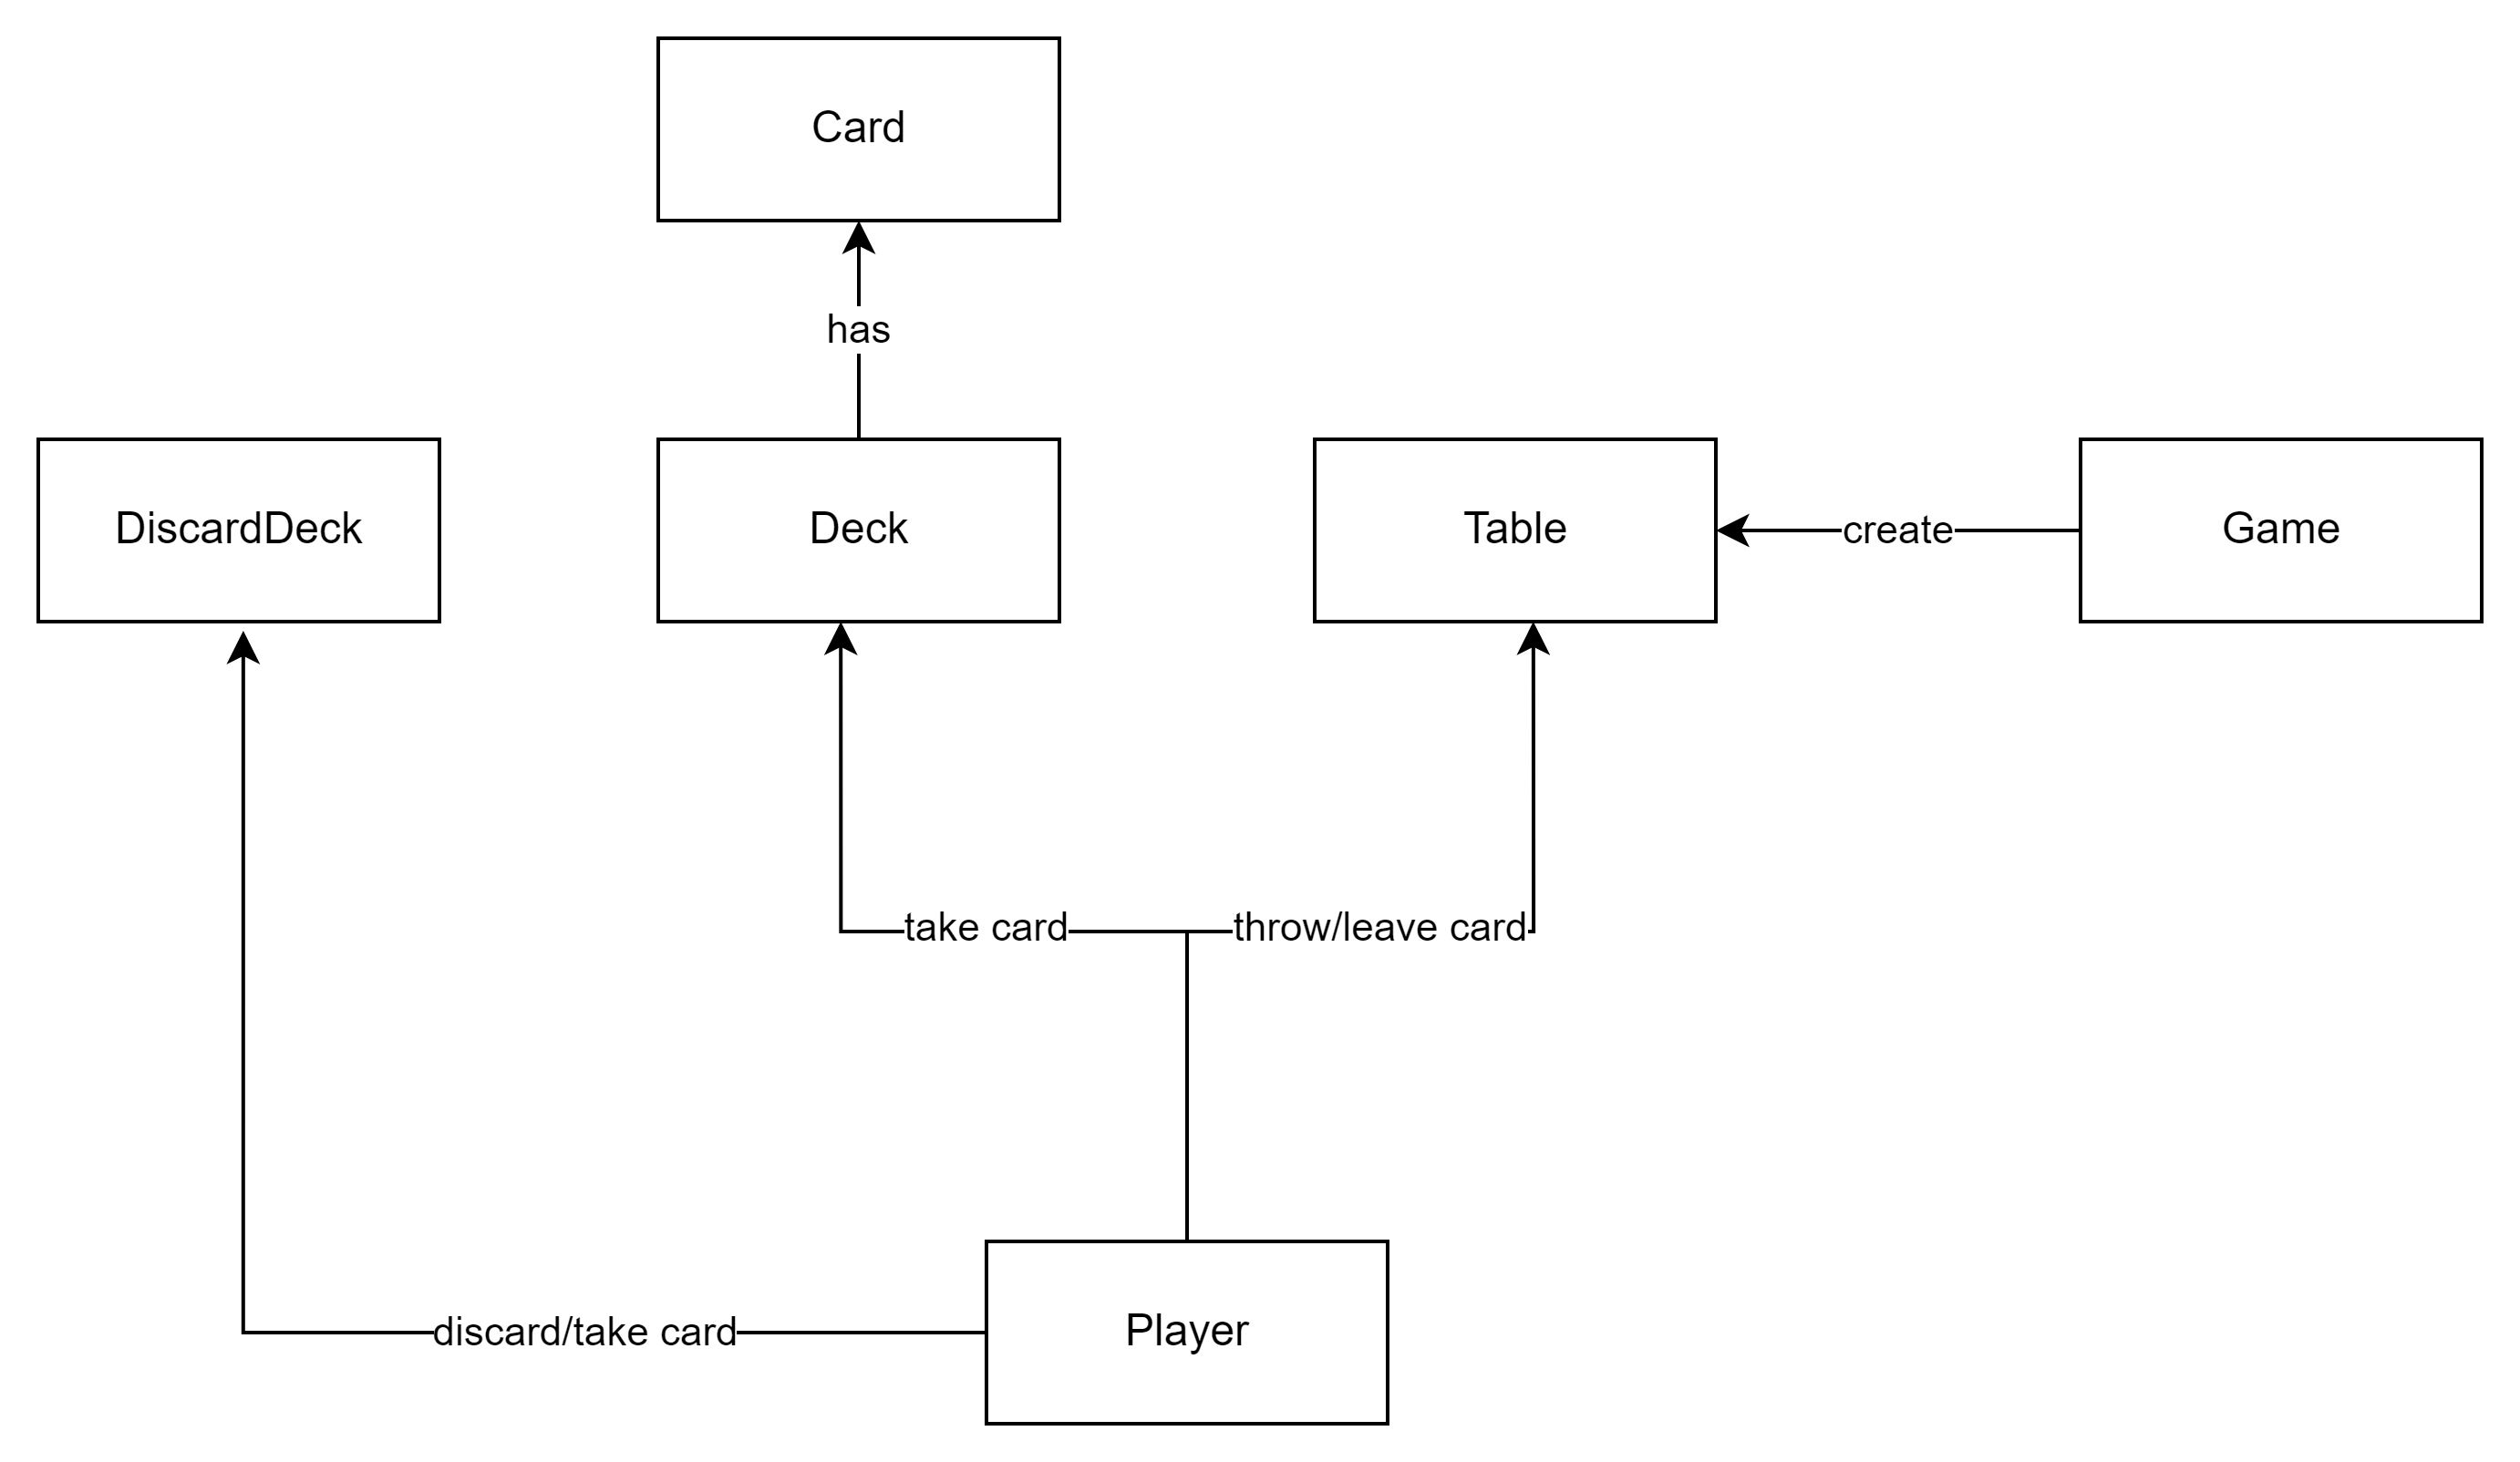
\includegraphics[width=15cm]{moobjetos.png}
    \caption{Modelo de objetos para el juego de cartas Cariocas.}
\end{figure}

\subsubsection{Diccionario de datos}\label{cap:diccionario-datos}
\begin{itemize}
    \item\textbf{Game}:Clase que se encarga de implementar las reglas y logica del juego, \\como tambien mostrar los datos necesarios por pantalla tal como el menu del sistema. 
    \item\textbf{Player}:Entidad que interactua con el juego, baraja y la baraja de descarte. Tiene la capacidad de tomar, dejar, botar cartas.
    \item\textbf{Card}:Clase para representar las cartas para el juego carioca, estas contienen un id, numero y pinta.
    \item\textbf{CardStack}:Clase Padre de Deck y DiscardDeck, la cual tiene como función almacenar instancias de la clase Card
    \item\textbf{Deck}:Clase hija de CardStack. Se almacenan instancias de la clase Cartas que son Generadas al principio del Juego
    \item\textbf{DiscardDeck}:Clase hija de CardStack. Se almacenan instancias de la clase Cartas que son descartadas por una instancia de la clase Player
    \item\textbf{Table}:Objeto de la clase Game, el cual almacena trios y escalas de los jugadores. 
\end{itemize}
\clearpage
\subsubsection{Diagrama de clases.}\label{cap:diagrama-clases}
A continuación se presenta el diagrama de clases del sistema a programar para el desarrollo del juego de cartas Cariocas:
\begin{figure}[H]
    \centering
    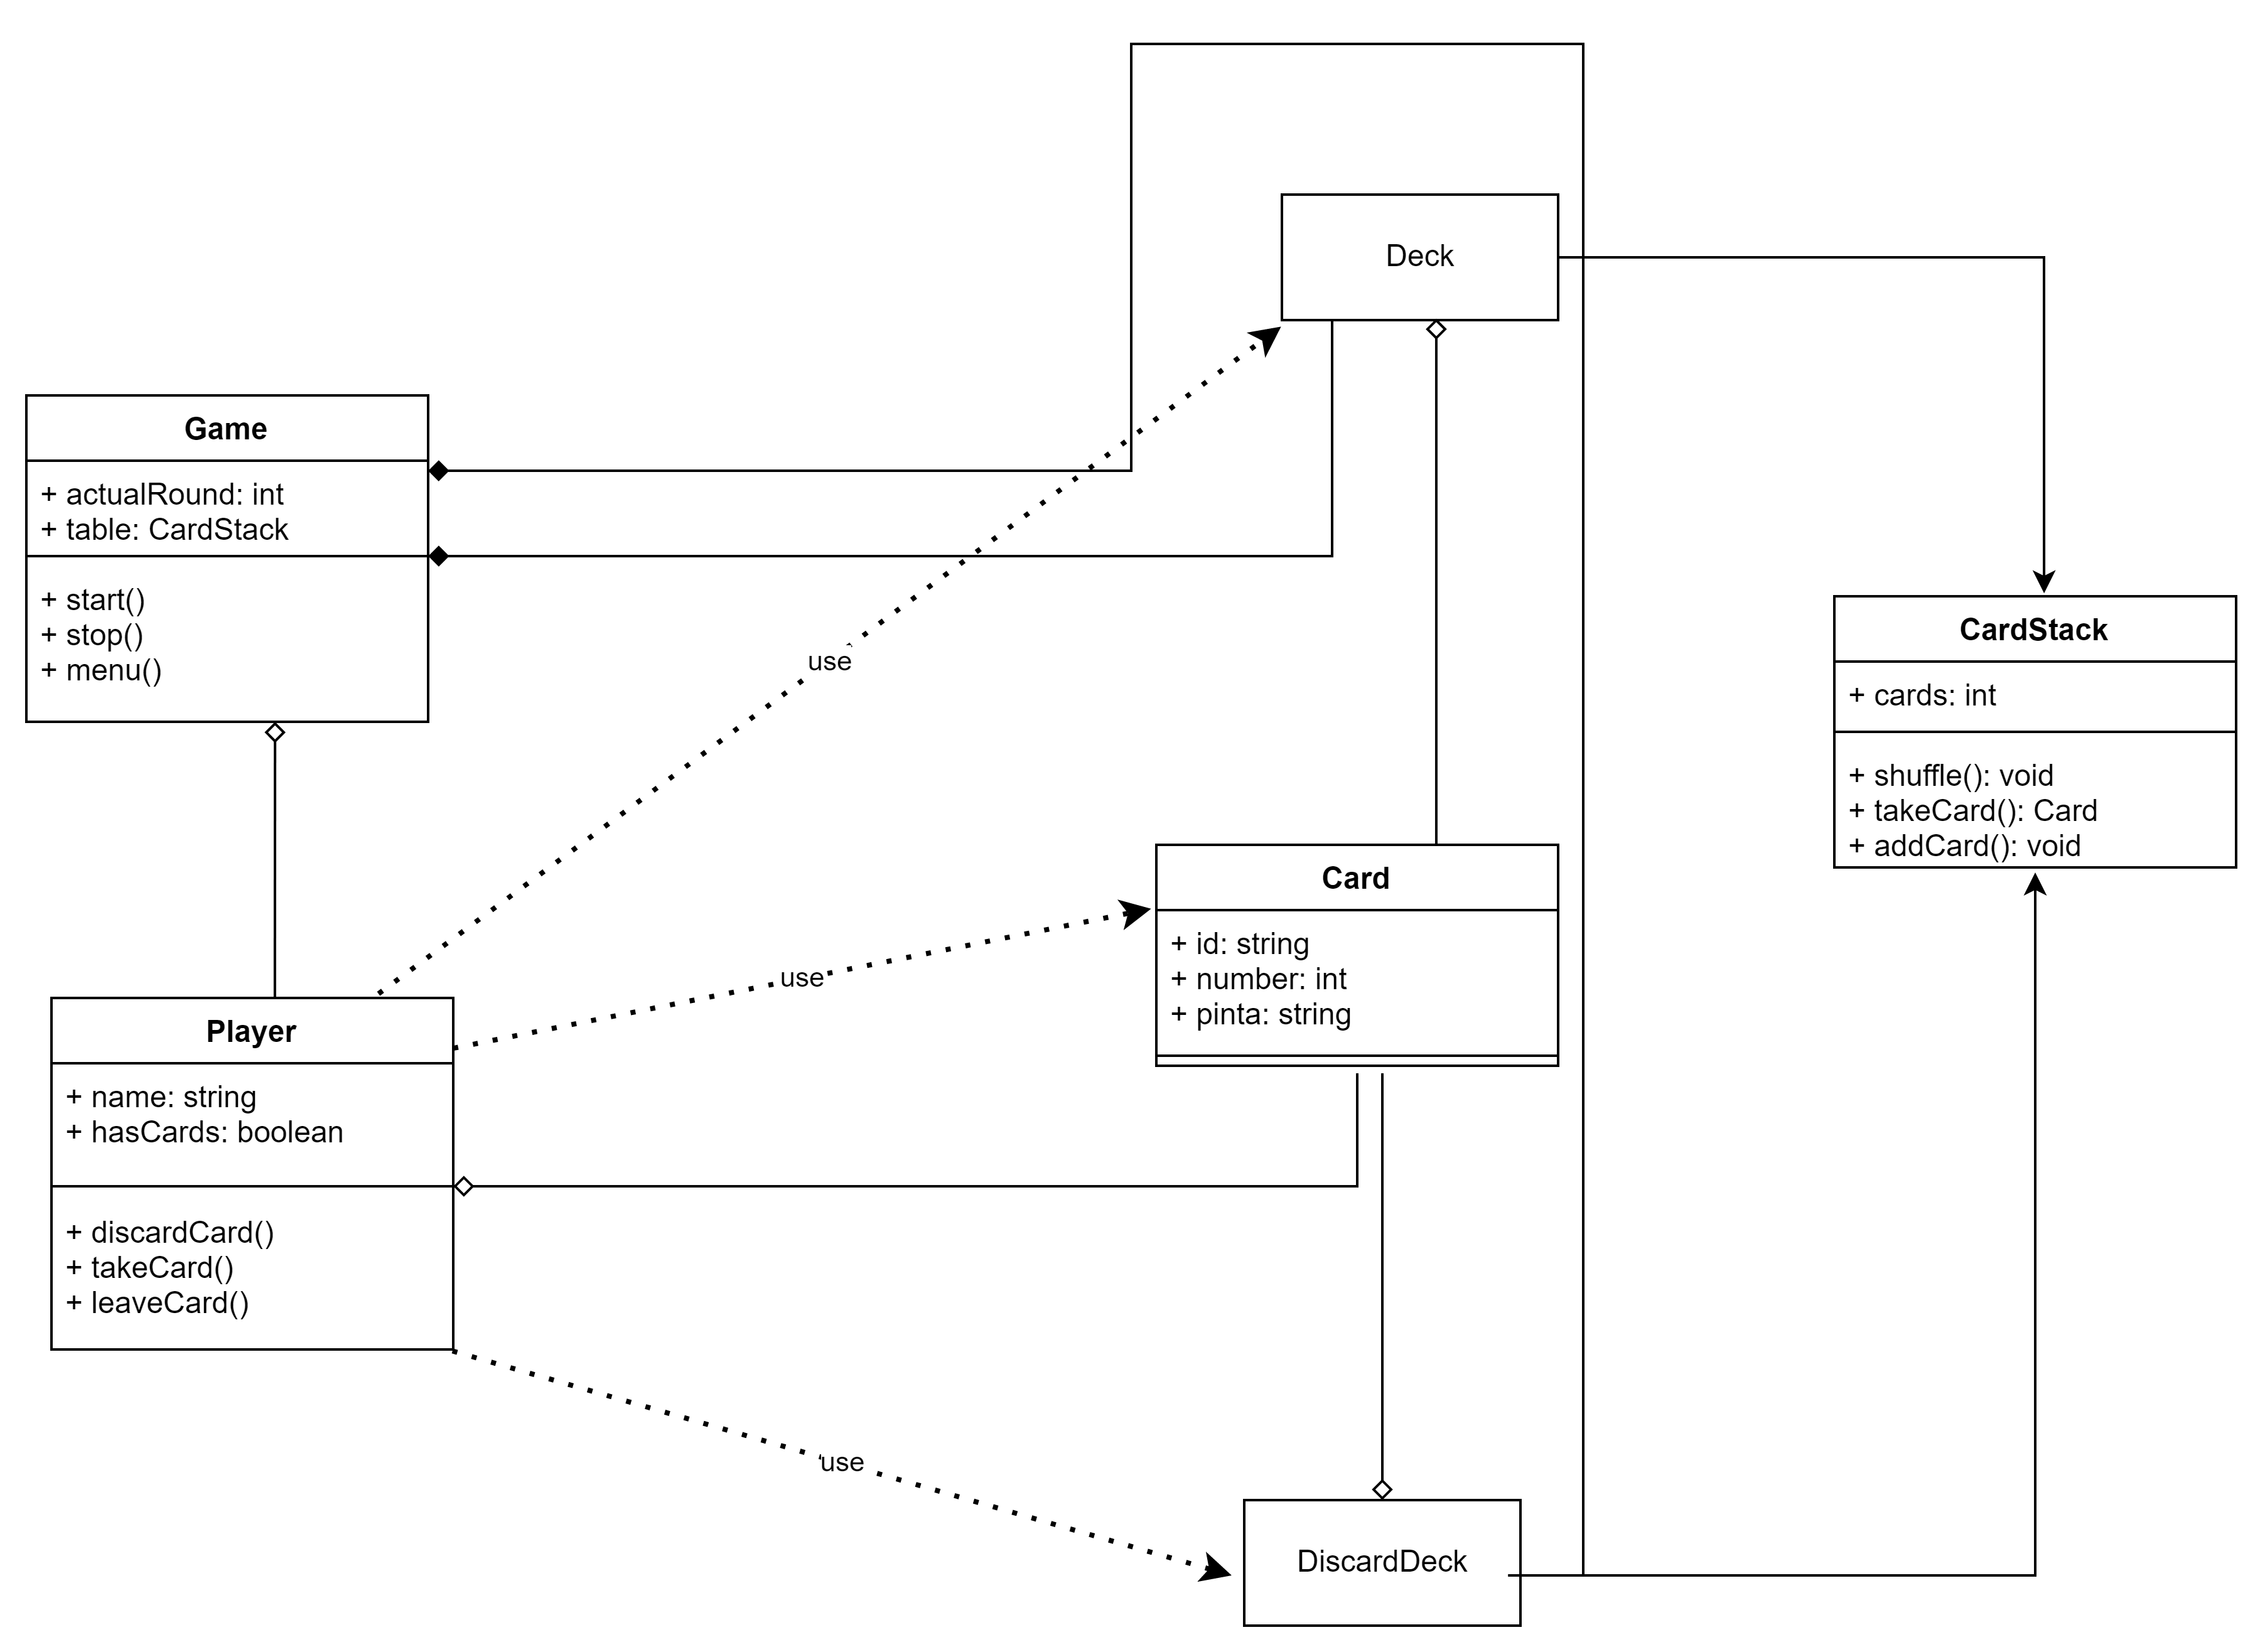
\includegraphics[width=15cm]{diclass.png}
    \caption{Diagrama de clases para el juego de cartas Cariocas.}
\end{figure}
\subsubsection{Interfaz de usuario}\label{cap:interfaz-usuario}
El siguiente diagrama muestra la interfaz de usuario del juego detallando así rutas de navegación y también maquetas de pantallas que tendrá el juego.
\begin{figure}[H]
    \centering
    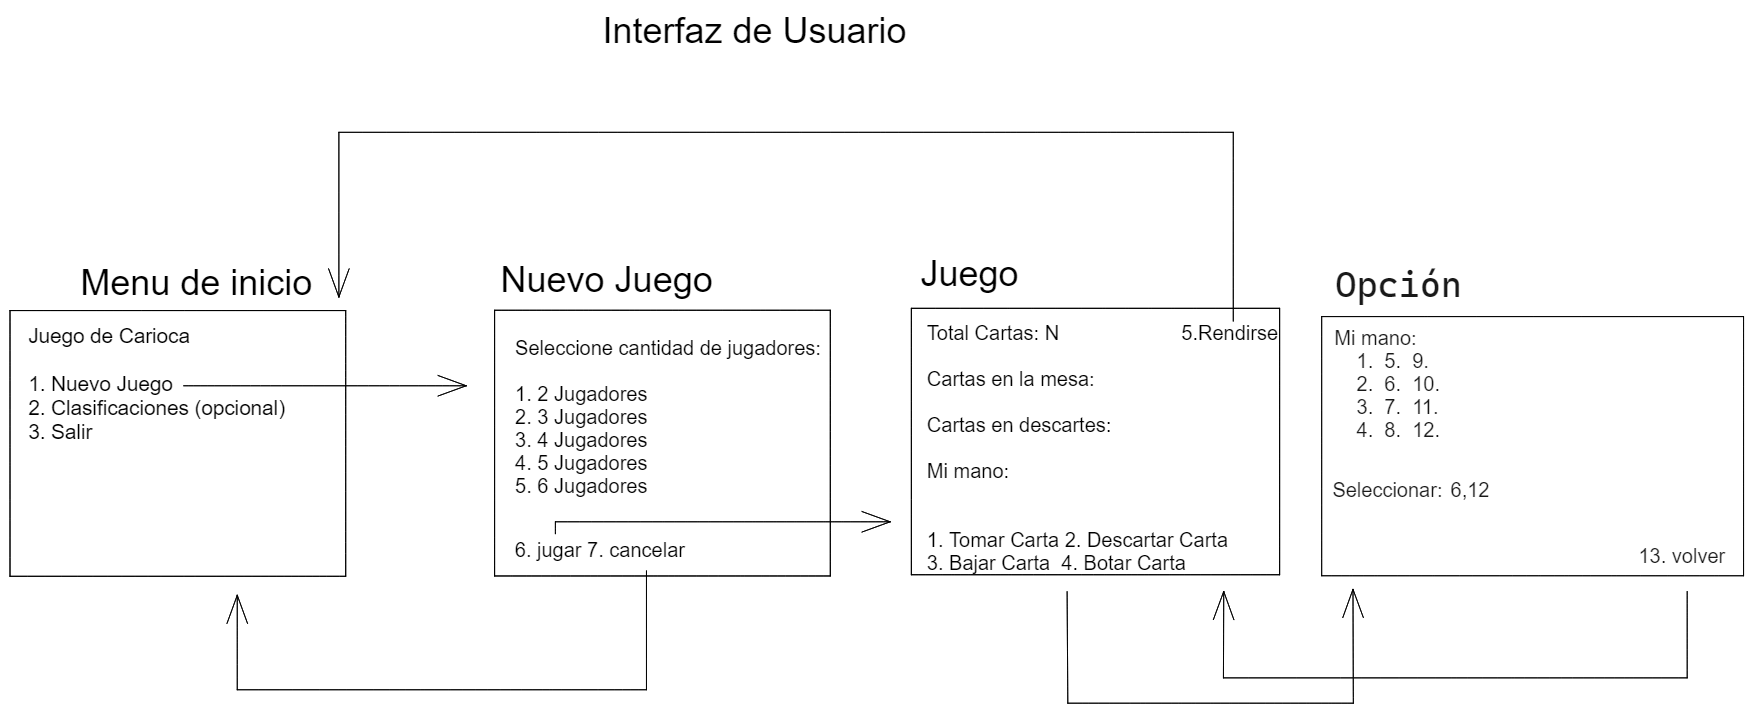
\includegraphics[width=15cm]{interfaz.png}
    \caption{Diagrama de interfaz de usuario para el juego de cartas Cariocas.}
\end{figure}
\clearpage
\section{Glosario}\label{cap:glosario}
\begin{itemize}
    \item \textbf{Patrón}: Conjunto de cartas que se deben completar.
    \item \textbf{Baraja}: Conjunto de cartas que se utilizan durante el juego.
    \item \textbf{Descarte}: Conjunto de cartas que se han descartado durante el juego.
\end{itemize}

\printglossary
\clearpage

\medskip
\printbibliography

\end{document}